%%%%
% -- Schedule and Budget breakdown and funding path
% --     FOBOS Keck White Paper 2019
%%%%

\section{Schedule, Budget, and Funding Path}
\label{sec:budget}

\subsection{Funding Path}

Early funding for FOBOS has been obtained as follows. Conceptual
development of Fiber-WFOS for TMT provided the backbone of the
current FOBOS design. Grants for targeted studies include: a 2016 UCO
mini-grant (K.-G.~Lee) for initial collaboration development; 2017
UCO mini-grants for microlens fore-optics conceptual development
(K.-G.~Lee) and the sky-subtraction fidelity of existing fiber
systems (K.~Bundy); WMKO 2018 white-paper funds (K.~Bundy; ongoing)
to develop science cases, build science teams, and perform
focal-plane and spectrograph design studies; and a 2018 UCO
mini-grant (K.~Bundy; {\it FIDDLES}, ongoing) to design and fabricate
a microlens-coupled fiber system to demonstrate its throughput at
Keck compared to lab measurements and to simultaneous observations
with DEIMOS. The latter builds on UCO's ongoing investment in a
fiber-testing facility needed for a number of internal projects has
helped to further the FOBOS design.

This Phase-A funding request is designed to bring the project to a
stage of readiness needed to submit proposals to the NSF MSIP (2020)
and MsRI-2 (2023) programs (see Table~1). We intend to propose for
FOBOS design funds via an MSIP solicitation expected in early 2020;
if successful, this will fund the full instrument-design phase. The
construction funding would then come from a MsRI-2 proposal in 2023.
The duration of our Phase-A request, late 2019 to mid 2021, will
allow for continued development between submitting our MSIP proposal
and when the funding is made available. In the event that we are
unsuccessful in the MSIP proposal, we will refocus Phase-A funding
during the latter half of this proposal period toward preparation of
an MsRI-1 proposal in 2021. Additional funding proposals for smaller
grants (e.g., UCO mini-grant, NSF ATI) will be sought as necessary
and available. These grants would target relatively self-contained
design components of FOBOS's overall system. Other government funding
and private funding is also being pursued as opportunities become
available.

\begin{table}[h!]
\centering
\footnotesize
\caption{FOBOS Development Milestones}
\label{tab:milestones}
\vspace*{-10pt}
\begin{tabular}{l r r}
Milestone                     & Funding Level & Dates \\
\hline
\hline
CoD Mini Grant I              &  \$10k & FY2016 \\
CoD Mini Grant II             &  \$25k & FY2017 \\
CoD Mini Grant III            &  \$55k & FY2017 \\
LBNL workshop                 &        & 18 Jan 2018 \\
UCLA workshop                 &        & 4 May 2018 \\
WMKO Design                   &  \$40k & 8 Jun 2018 \\
WMKO Design Funding Window    &        & 1 Dec 2018 -- 30 Nov 2019 \\
CoD Mini Grant IV (FIDDLES)   & \$120k & FY2019 \\
FIDDLES Funding Window        &        & 10 Jan 2019 -- 11 Dec 2019 \\
\hline
MSRI-1 Proposal               &        & 19 Feb 2019 \\
WMKO Phase A                  & \$376k & 8 Jun 2019 \\
WMKO Phase A Funding Window   &        & 23 Sep 2019 -- 23 Jul 2021 \\
\hline
MSIP 2020 LOI, Pre-Proposal   &        & 1 Sep -- 18 Nov 2019 \\
MSIP 2020 Full Proposal       &   \$5M & 17 Apr 2020 \\
MSIP Funding Window           &        & 1 Sep 2020 -- 31 Aug 2024 \\
\hline
MSRI-2 LOI, Pre-Proposal      &        & 16 Feb -- 13 Mar 2023 \\
MSRI-2 Full Proposal          & $>$\$20M & 4 Aug 2023 \\
MSRI-2 Funding window         &        & 1 Aug 2024 -- 31 Sep 2028 \\
\hline
\end{tabular}
\end{table}

\newpage

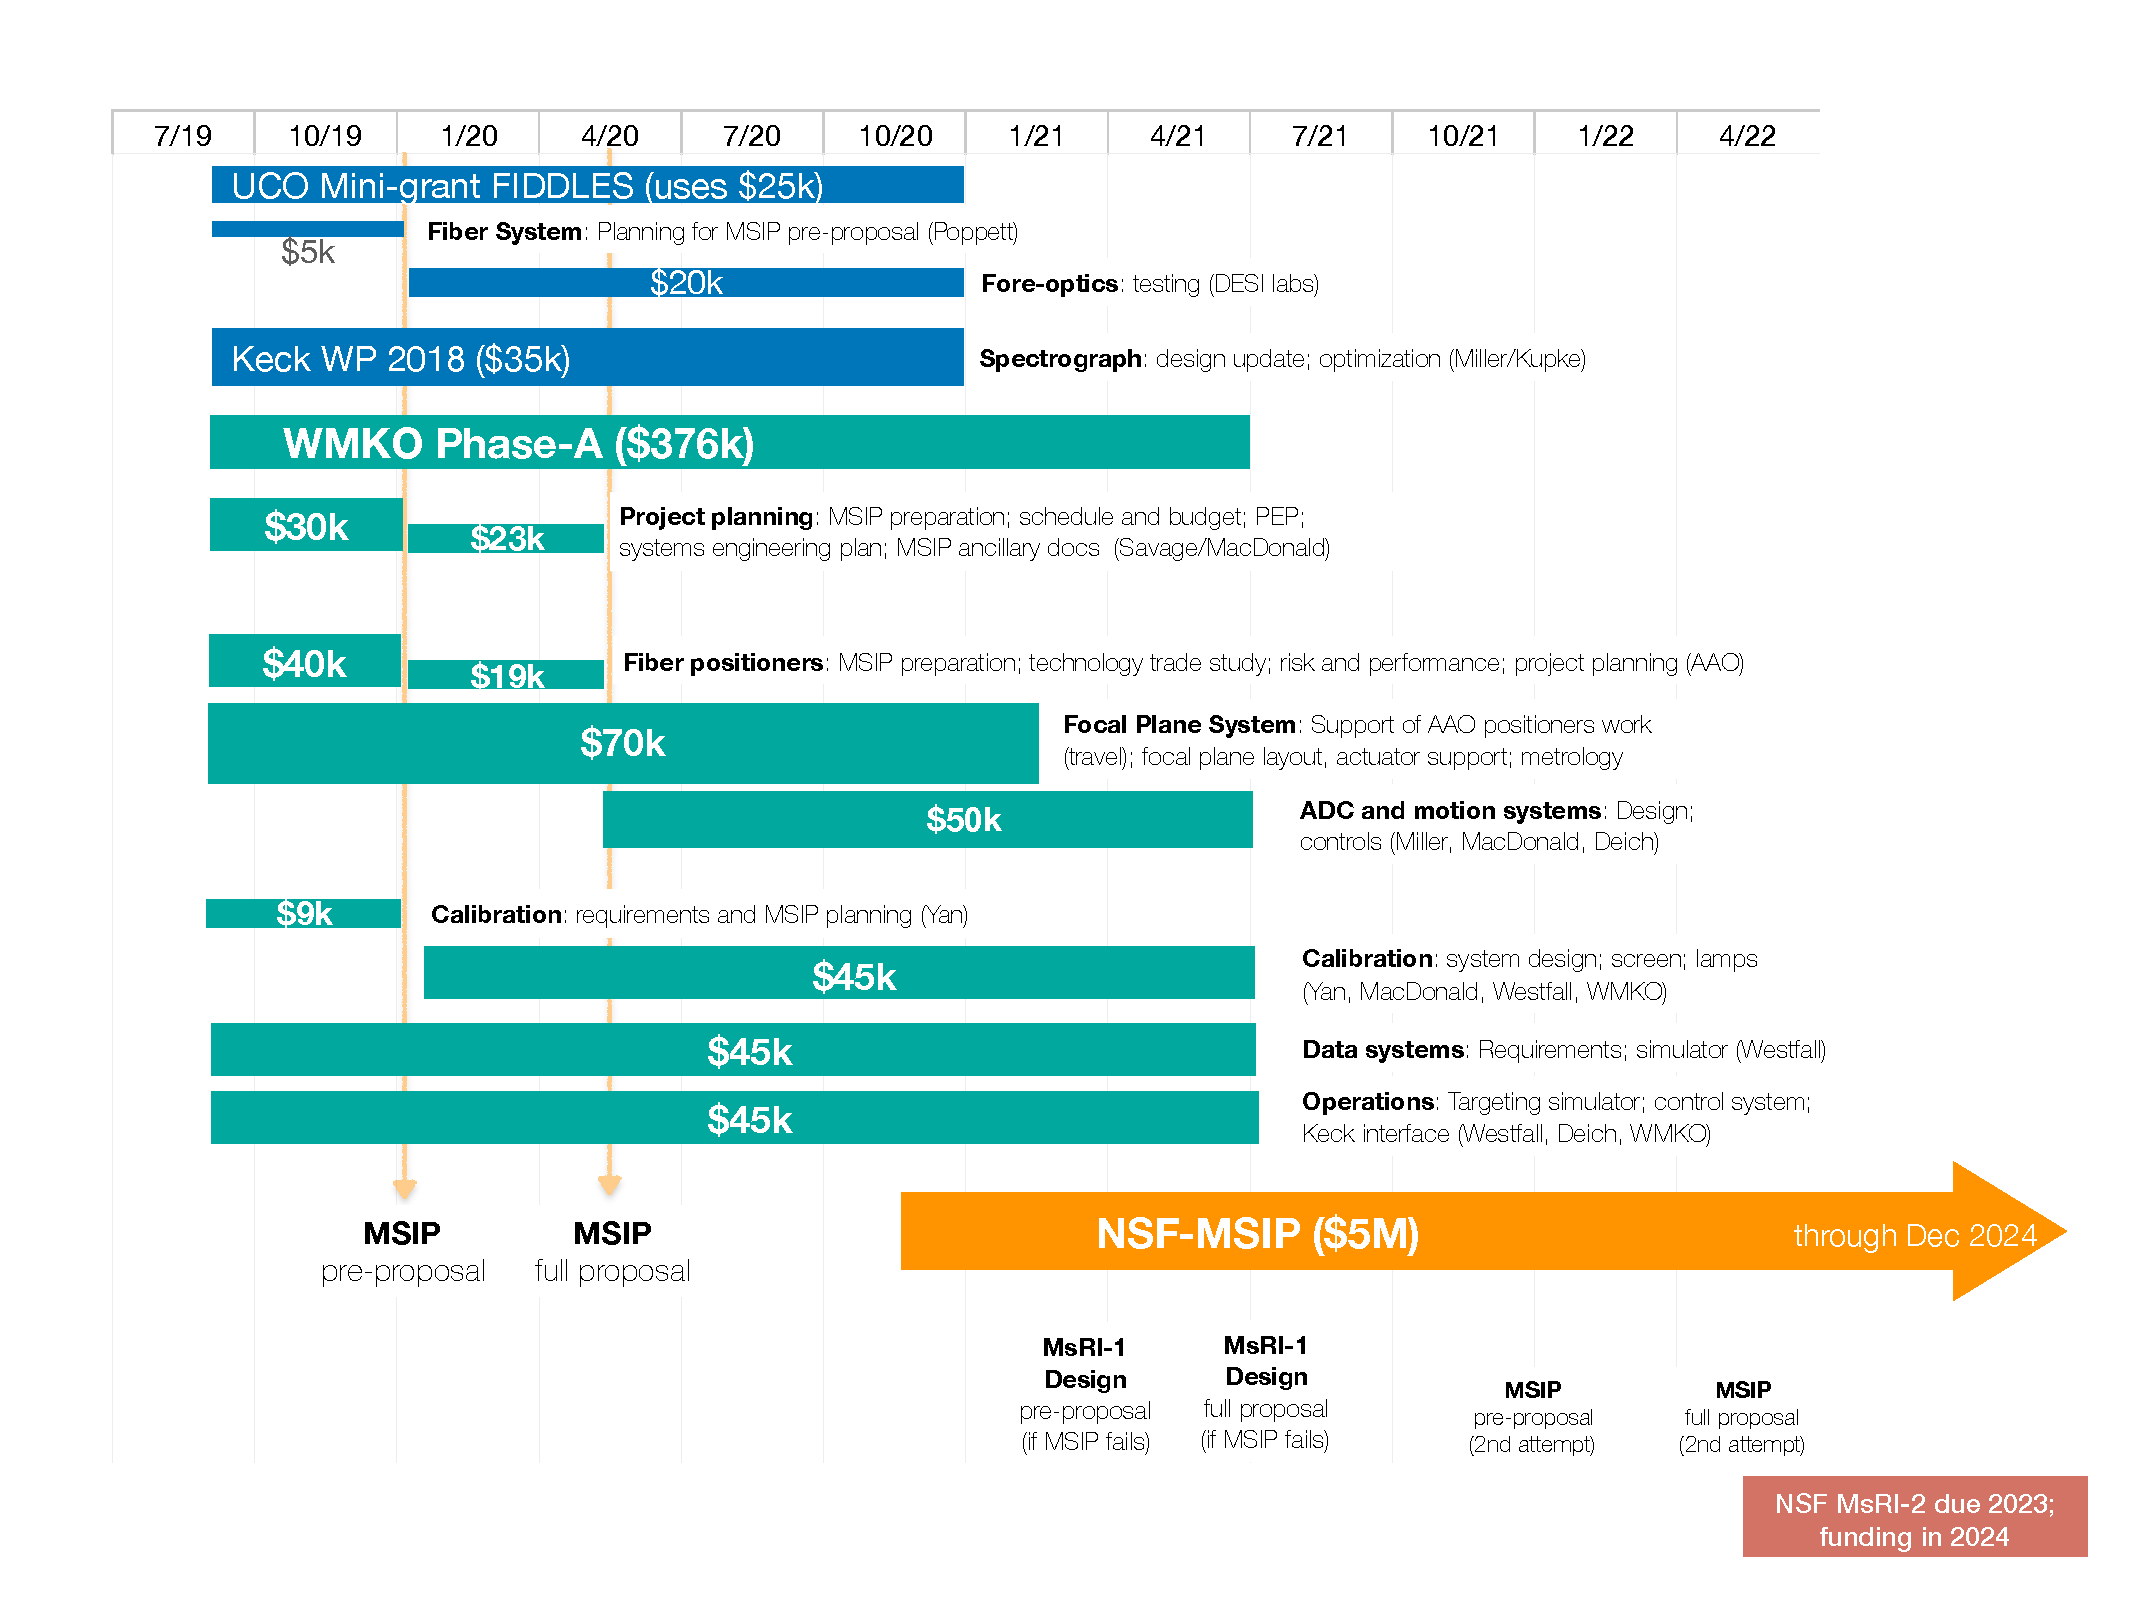
\includepdf[landscape=true]{figs/budget_schedule_schematic_v3.pdf}





